\chapter{实验结果与分析}
本章节主要是对此前在UPMEM上进行软硬协同优化的GEMV算子的综合测试,第一小节介绍环境配置平台,第二小节重点在UPMEM近存计算硬件平台上进行算子综合测试,包括与其他常见的硬件计算平台进行对比,第三小节重点在PIMulator模拟器平台上测试硬件优化的效果。

\section{环境配置介绍}

\subsection{硬件平台}
本文实验的近存计算平台在UPMEM官方推荐的UPMEM服务器上。该服务器配备了双插槽的英特尔至强4210 CPU,每颗CPU拥有10个核心20个线程,每个核心工作在2.20GHz的基准频率,拥有32KB的L1缓存、1MB的L2缓存和13.75MB的L3缓存。每个CPU配备6个内存通道,支持DDR4-2400的内存。我们为每个CPU的5个通道插满UPMEM DIMM,剩余的一个通道配置常规DDR4-2400的内存。每个内存通道插入两根UPMEM DIMM,每个UPMEM DIMM上配有128个DPU。因此一共有$2\times 5\times 2\times 128=2560$个DPU可以同时工作,每个DPU的存储容量为64MB,因此UPMEM内存的存储容量一共是160GB。普通CPU内存有128GB。

同时实验对比使用的CPU平台是在配备了双插槽的英特尔至强6242 CPU的服务器平台上,每颗CPU拥有16个核心32个线程,每个核心工作在2.80GHz的基准频率,拥有32KB的L1缓存、1MB的L2缓存和22MB的L3缓存。每个CPU配备6个内存通道,支持DDR4-2933的内存。该平台上没有插UPMEM DIMM,全部配备的是标准DDR4内存共256GB。之所以CPU平台和UPMEM平台要分开成两套硬件测试,而不能复用UPMEM平台的原因是,UPMEM平台的CPU的6个内存通道有5个都被UPMEM占用,CPU内存传输带宽变为原来的六分之一,这样的对比实验并不公正。

GPU的硬件装配在CPU平台上,由于通过PCIE接口连接而并不影响性能。GPU平台配备了一块Nvidia A6000 GPU,其核心代号为GA102,安培架构,拥有10752个CUDA Core和336个Tensor Core,单精度浮点性能达38.7TFLOPS。其拥有48GB的GDDR6显存,384bit的传输位宽,显存带宽能达到768GB/s,足以容纳我们评估中使用的数据。具体详细的硬件配置可以见表\ref{ExpConfig}。

\begin{table}[!htbp]
	\centering
	\caption{硬件平台配置}
	\label{ExpConfig}
	\resizebox{\textwidth}{!}{
		\begin{threeparttable}
			\begin{tabular}{|c|c|c|c|c|c|c|c|c|}
				\hline \multirow{2}{*}{硬件平台} & \multirow{2}{*}{$\begin{array}{l}\text {制程}\end{array}$} & \multicolumn{3}{|c|}{处理核心} & \multicolumn{2}{|c|}{内存} & \multirow{2}{*}{功耗} \\
				\cline{3-7} ~ & ~ & $\begin{array}{l}\text {核心数}\end{array}$ & 工作频率 & $\begin{array}{l}\text{峰值性能}\end{array}$ & $\begin{array}{l}\text{容量}\end{array}$ & $\begin{array}{l}\text {总带宽}\end{array}$ & ~\\
				\hline Intel Xeon 6242 CPU& $14 \mathrm{~nm}$ & $16$ & $2.8 \mathrm{GHz}$ & 89.6 GFLOPS & $255.9 \mathrm{~GB}$ & $256 \mathrm{~GB} / \mathrm{s}$ & $150 \mathrm{~W}$ \\
				\hline NVIDIA A6000 GPU& $8 \mathrm{~nm}$ & $\begin{array}{l}10752\end{array}$ & $1.41 \mathrm{GHz}$ & $38.7$ TFLOPS & $48 \mathrm{~GB}$ & $768 \mathrm{~GB} / \mathrm{s}$ & $300 \mathrm{~W}$ \\
				\hline UPMEM& $2 \mathrm{x}\;\mathrm{nm}$ & $2560$ & $400 \mathrm{MHz}$ & 1024 GOPS & $160 \mathrm{~GB}$ & $1.7 \mathrm{~TB} / \mathrm{s}$ & $256 \mathrm{~W}$ \\
				\hline
			\end{tabular}
			% \begin{tablenotes}
			% 	\item[1] $2.8GHz \times 16\;cores \times 2 \;inst \;per \;cycle = 89.6 GFLOPS$
			% 	\item[2] $2666MHz\times 64\div 8 Byte \times 6 = 127.968GB/s$
			% 	\item[3] $400MHz \times 2560\;cores \times 1 \;inst \;per \;cycle = 1024 GOPS$
			% 	\item[4] $12.8W \;per \;DIMM \times 20 = 256W$
			% \end{tablenotes}
		\end{threeparttable}
	}
\end{table}

\subsection{数据准备和矩阵尺寸选择}
本文选择被广泛使用的开源模型Llama2-7b-chat,使用WikiText2\footnote{https://huggingface.co/datasets/mindchain/wikitext2/tree/main}和PTB\footnote{https://aistudio.baidu.com/datasetdetail/67}作为量化校准数据集对原始权重进行FP8/FP4量化,以随机选取的量化后的权重矩阵(MHSA中的线性层)作为测试数据。我们在主要的测试中选取的GEMV数据尺寸为$4096\times 1024$,对应Llama2-7B推理过程中的线性层;在扩展性测试中我们将使用不同矩阵尺寸测试DPU的扩展性。在数据宽度方面,近存计算平台选择FP8(E4M3)数据格式进行测试,在CPU和GPU平台选择Float32进行测试(精度由现有量化方法工作保证)。每个DPU使用$4096\times 1024$尺寸的矩阵,用满UPMEM所有DPU进行总的吞吐测试,矩阵的大小为$4096\times 1024\times 2560$,假设使用FP32的数据格式,矩阵所占空间最大为$4096\times 1024\times 2560\times 4Byte=40GB$,上述硬件平台足以存储。

\subsection{基线设置}
对于商用近数计算硬件平台的测试,我们设置基线(baseline)分别为CPU、GPU和UPMEM平台的Float32矩阵向量乘。PIM平台使用UPMEM SDK(版本 2024.1.0)编译在UPMEM-DIMM执行;CPU平台使用英特尔数学核心函数库(Intel Math Kernel Library,MKL)\cite{IntelMKL},它是英特尔官方开发的一套高性能数学计算库,里面包含BLAS接口,针对Intel(至强处理器)硬件特性进行了深度优化(包含OpenMP以及SIMD指令),同时能够简单高效地支持多线程和并行计算;而GPU平台我们将基于CUDA(12.2)使用cuBLAS库\footnote{https://docs.nvidia.com/cuda/cublas/index.html}:cuBLAS是NVIDIA官方开发的一个高性能线性代数库,专为CUDA平台设计,充分利用了NVIDIA GPU的硬件特性,能够显著加速矩阵乘法(GEMM)、向量运算和其他线性代数任务。对于下发的任务包括GEMV,在支持Tensor Core的GPU硬件上,cuBLAS会自动优化选择使用Cuda Core还是Tensor Core以到达最佳性能。对于近存计算模拟器平台的测试,我们主要测试硬件修改对算子的提升,基线设置为第三章提出的三个算法LUT-M\ref{LUT-M}、LUT-W-R\ref{LUT-W-R}和LUT-W-C\ref{LUT-W-C}以及朴素GEMV内积LUT-FP4。

\section{基于近存计算平台的软件优化测试与分析}

\subsection{总吞吐对比测试}
我们定义GEMV算子的吞吐为每秒操作运算次数(Operations Per Second, OPS)来衡量,对于矩阵尺寸为$M\times N$的GEMV算子来说,具体的计算公式为\ref{GOPsEqu},其中$M\times N$的矩阵中的每个元素都要进行一次乘法和加法,因此是两次操作;ExecuteTime为GEMV算子的多次连续执行的平均耗时,单位为秒。图\ref{EXP1-1}分别显示了在近存计算平台(UPMEM)、CPU平台和GPU平台上的GEMV算子运算性能,UPMEM使用了全部2560个DPU,每个DPU配置16个tasklet,LUT-W-R算法配置子矩阵大小为$32\times 512$。

\begin{equation}
    Throughput=\frac{2\times M\times N}{ExecuteTime}\times 10^{-9}\; GOPS
    \label{GOPsEqu}
\end{equation}

\begin{figure}[!htbp]
    \centering
    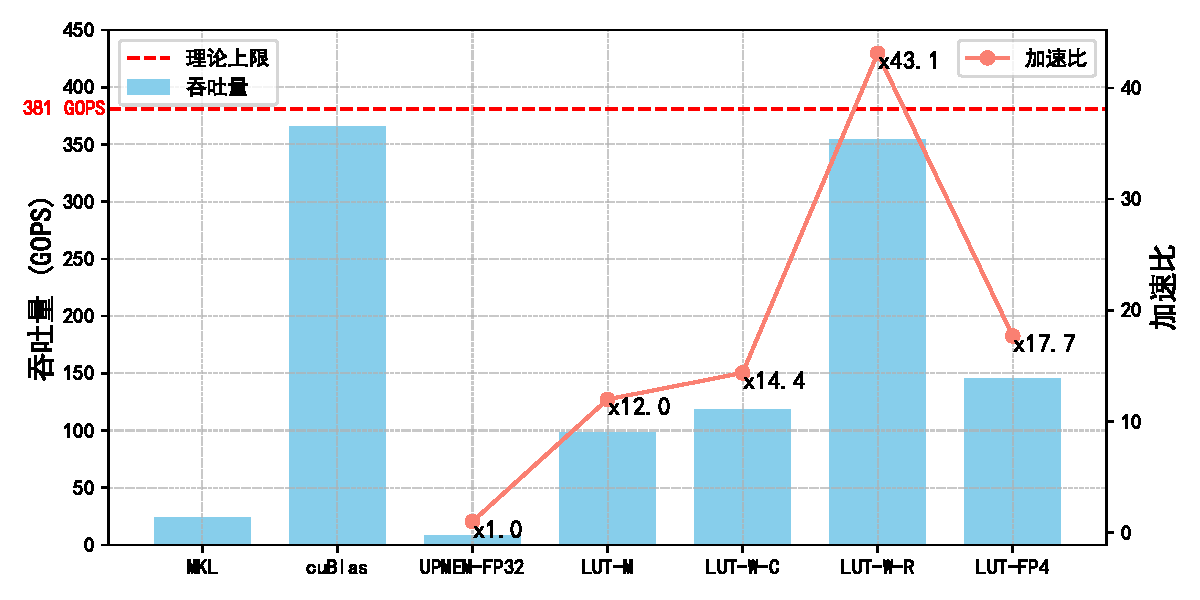
\includegraphics[width=0.9\textwidth]{figures/Exp1-1.pdf}
    \caption{不同平台及算法下GEMV总吞吐}
	\label{EXP1-1}
\end{figure}

结果显示,与CPU平台的MKL库中的矩阵向量乘法相比,UPMEM平台的最大吞吐算法LUT-W-R算法有14.7倍的提升,而相比较GPU的cuBlas而言,吞吐量基本持平有微小的差距。CPU平台使用MKL库充分利用了Intel CPU的向量指令和多线程(OpenMP,设置线程数量为16)并行计算,但是由于CPU平台有限的内存带宽和复杂的存储层级,GEMV受到数据传输的限制,性能与近存计算平台相差较大。对于GPU的表现符合预期,因为GPU的内部带宽并不低,此前在第四章的分析中发现UPMEM平台的内存带宽利用率最高也只达到10\%左右,因此二者在数据传输方面的表现是类似的。同时GPU的核心数量并不少,且每个核心的主频更是有1.41GHz是UPMEM的核心主频的2~3倍,因此理应相较于UPMEM更快,但是UPMEM平台凭借着高速的内部带宽和精调的优化算法缩小了与GPU平台的差距。同时在GPU测试的过程中,我们发现计算吞吐(Compute SM Troughput)仅达47.57\%,远远没有充分利用硬件计算的能力,然而内存带宽利用率却以及达到96.89\%表现为内存瓶颈。

同时可以看到在UPMEM平台上,软件优化的加速比。以最基础的GEMV算法UPMEM-FP32为基准,该算法就是普通地使用UPMEM上的软件模拟Float32直接进行计算而不采用查找表,其性能非常低,吞吐仅达8GOPS。使用了针对MRAM的分块载入查找表的算法LUT-M后,相比UPMEM-FP32有巨大的提升,加速比高达12倍。之后是针对WRAM优化的两种算法将矩阵行重排LUT-W-R和矩阵列重排LUT-W-C。在这之中,LUT-W-C的算法的提升有限,达到UPMEM-FP32的14.4倍,而LUT-W-R算法提升较高,是各种软件优化算法中吞吐最高的算法,达到355GOPS,是UPMEM-FP32的43.1倍。LUT-FP4的算法是卸载W4A8量化的矩阵向量乘法,因为权重进一步量化到了4bit,因此乘法查找表的大小刚好只有16KB,完全能够放在WRAM中,因此执行的算法与UPMEM-FP32是类似的,同样是矩阵向量的内积,只不过乘法换成了查表操作。此处比较奇怪的是,LUT-FP4算法虽然相比UPMEM-FP32算法有17.7倍的提升,但是却弱于LUT-W-R算法,而LUT-W-R算法是载入子矩阵同样进行内积操作,理应比LUT-FP4要更慢。我们通过研究两种算法的汇编代码后发现,LUT-W-R的算法汇编代码进行了循环展开而LUT-FP4完全没有展开,换言之LUT-W-R的编译优化非常好,性能远超LUT-FP4(在第三小节的测试也侧面说明了这一点),因此出现了LUT-FP4算子吞吐弱于LUT-W-R的情况,推测主要原因在于UPMEM的软件栈不够完善。

同时为了评估硬件限制对UPMEM平台的影响,将LUT-W-C算法下的GEMV的实际性能与理论性能进行了比较。理论性能通过公式\ref{MaxThroughput}计算。其中$N_{dpu}$表示 UPMEM核心的数量,为2560。$F$表示核心频率,为400MHz。$N_{inst}$表示执行一次FMA操作所需的指令数,包括5条指令:1条用于加载权重,1条用于地址生成,1条用于乘法,1条用于加法,以及1条用于循环中的杂项操作。理论带宽上限为381GOPS,测试的LUT-W-C算法的GEMV算子吞吐为355GOPS,大概达到理论性能的93\%。

\begin{equation}
    MaxThroughput=\frac{2\times N_{dpu}\times F}{N_{inst}}\; GOPS
    \label{MaxThroughput}
\end{equation}

\subsection{能效比测试与瓶颈分析}
近存硬件平台的一大优势在于其减少了数据移动的开销从而能够更加节能,非常适合边端对功耗有严格要求的设备,因此我们在测试计算能力的同时也测试了各个硬件平台的能效比。我们使用Intel VTune Profiler来测试CPU平台上的能耗,同时使用Nsight工具来测试GPU平台的能耗。对于UPMEM平台,由于官方没有提供能耗测试工具,因此我们只能通过UPMEM SDK的dpu-diag工具测试DPU的内核和DRAM Bank的静态功耗,大约为12.8w每根DIMM条。能效比定义简单地计算公式为\ref{EnergyEffiency},其中算子吞吐与上一小节中的测试结果保持一致,Energy为能耗,单位瓦特(W)。

\begin{equation}
    EnergyEffiency=\frac{Troughput}{Energy}\; GOPS/W
    \label{EnergyEffiency}
\end{equation}

能效比的实验如图\ref{EXP1-2:1}所示,其中以CPU平台的能效比作为基准(1),对其他平台和算法的能效比进行了测试和数据整理,可以看到除了UPMEM-FP32算法因过低的算子吞吐导致能效比较低外,其他平台的能效比皆高于CPU平台,其中最高能效比的算法为LUT-W-R,是CPU平台的8.6倍,是GPU平台的1.13倍,结果充分显示了近存计算平台的低能耗的优势。

\begin{figure}[htbp!]
	\centering
	\subfigure[能效比实验]{
		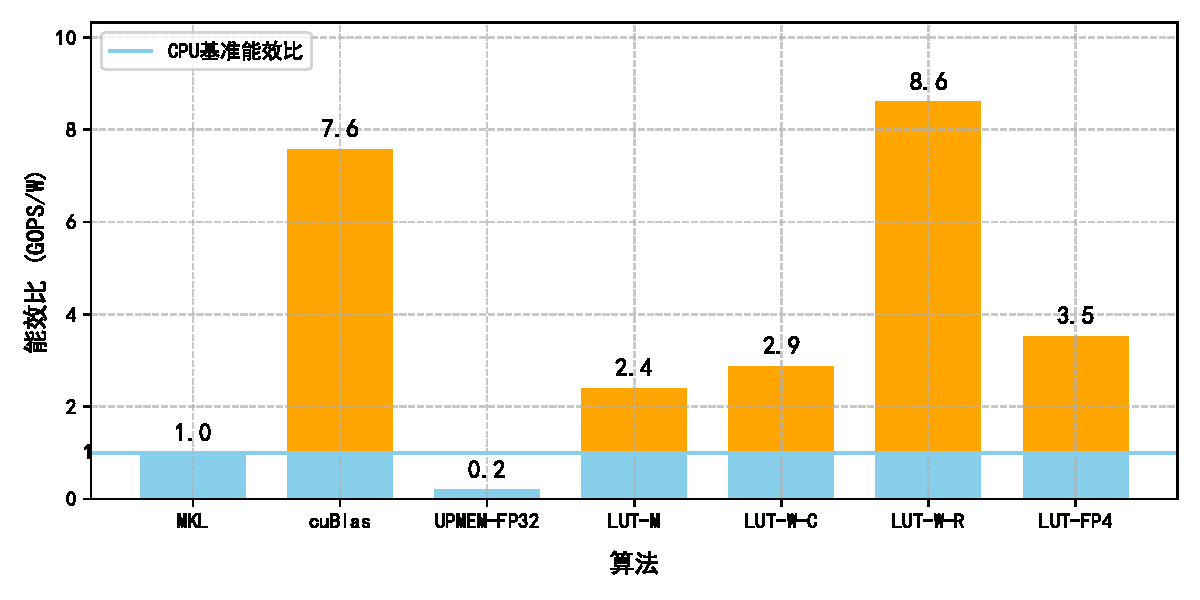
\includegraphics[width=0.9\linewidth]{figures/Exp1-2-1.pdf}
		\label{EXP1-2:1}}
	\\
	\subfigure[瓶颈分析]{
		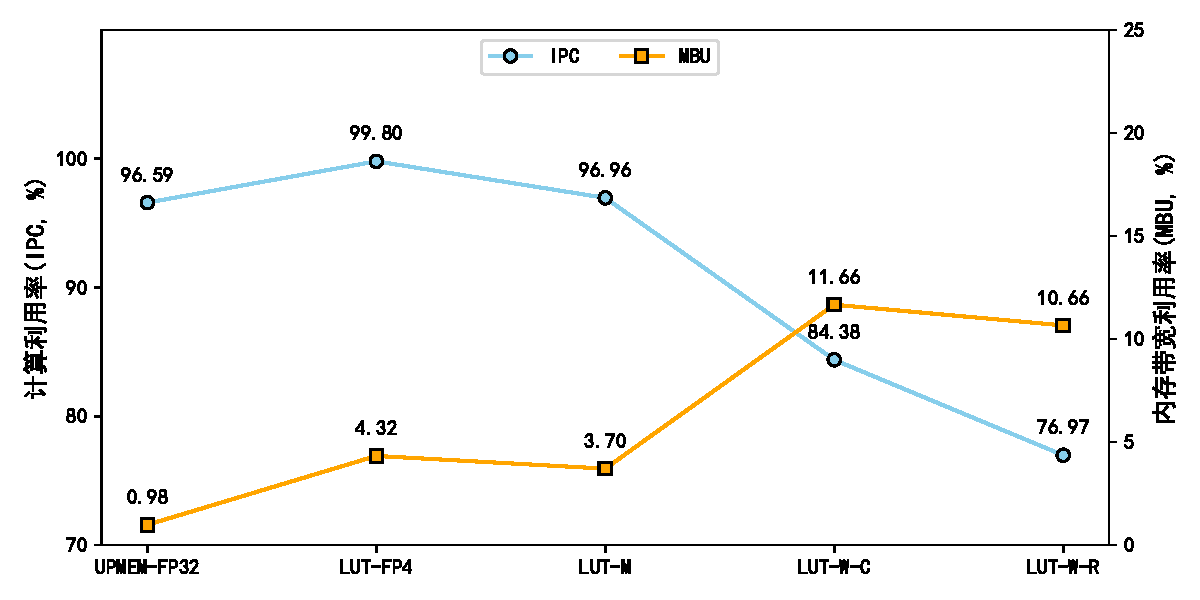
\includegraphics[width=0.9\linewidth]{figures/Exp1-2-2.pdf}
        \label{EXP1-2:2}}
	\caption{不同平台及算法下GEMV能效比和瓶颈分析}
	\label{EXP1-2}
\end{figure}

同时在这里对第四章的表\ref{BottleneckTable}进行补充测试,完善了UPMEM平台下各种算法的计算利用率和内存带宽利用率的数据如图\ref{EXP1-2:2}所示,此时矩阵的大小为$4096\times 4096$,设置16个Tasklets,LUT-W-R算法配置子矩阵大小为$32\times 64$。此前已分析过CPU平台和GPU平台都是内存瓶颈,反观UPMEM平台的各种算法,IPC都相当之高而内存带宽利用率仅最高达11\%,是非常明显的计算瓶颈的表现。同时可以看到逐步优化算法会将IPC降低而MBU提高,是非常典型的使用访存减少计算的优化手段,这意味着在UPMEM这种近存平台编程或者加速应用需要转变此前的冯诺依曼架构计算机的编程定式——减少访存,在近存平台上访存变得更加的“便宜”,我们往往需要用访存换计算。

此外实验中比较特殊的点在于LUT-FP4相较于LUT-M,从MRAM读写的字节数量是相同的(FP4仍然用8bit存储减少取数的开销),但是由于LUT-FP4能够执行GEMV内积而LUT-M只能执行GEMV外积导致LUT-FP4的WRAM访问更少,因此运行时间更短,IPC更高且MBU更高。

\subsection{扩展性测试}
本小节将从两个方面对算法进行扩展性测试,首先测试UPMEM每个DPU中的多线程扩展性,即保持矩阵的尺寸不变,增多Tasklet数量,观察算法性能。另一个方面,我们将测试算法处理矩阵尺寸的扩展性,即保持Tasklet的数量不变,增大矩阵的尺寸观察算法的性能。

对于多线程扩展性,本小节测试的矩阵大小为$4096\times 4096$,具体的算法选择以下几种:UPMEM-FP32,LUT-FP4,LUT-M,LUT-W-C,LUT-W-R。设置Tasklet数量从1逐渐翻倍到16,测试各个算子的执行时间如图\ref{EXP3-1}所示。可以看到无论是哪种算法,随着Tasklet的成倍增加,各个算法的执行时间随之成倍减少(对数坐标),然而当Tasklet的数量从8变化到16时,执行时间只减少到了原来的1.3倍,这个刚好符合从8变化打11扩大1.3倍的数据对应关系,也同样验证了UPMEM的流水线在11个线程时就已经充满,多增加线程无继续提升计算吞吐的硬特性。

\begin{figure}[htbp]
    \centering
    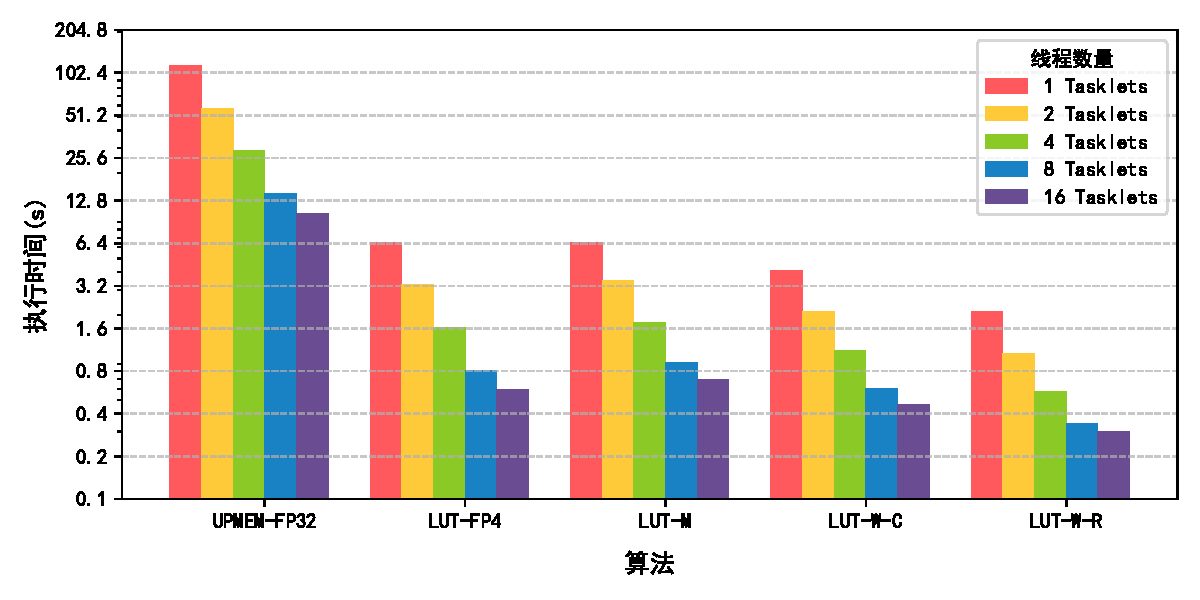
\includegraphics[width=0.9\textwidth]{figures/Exp3-1.pdf}
    \caption{UPMEM平台不同GEMV算法的多线程扩展性测试}
	\label{EXP3-1} %% label for entire figure 
\end{figure}

在Llama2-7B的MHSA中,会将一个完整的4096长度的词向量通过线形层成映射到32个子空间,对应到32个头(会将$4096\times 1$的向量映射成32个$128\times 1$的向量),本质上属于降维操作,(单个头)线形层是一个$4096\times 128$的窄矩阵;在最终计算得到attention向量后,又会通过一个线性层将$128\times 1$的向量重新映射为$4096\times 1$并最终合并各个头的结果,属于升维操作,此时线形层是一个$128\times 4096$的宽矩阵。同时由于DPU的通信开销低的特性,往往对算子进行融合,比如将QKV的单个头的线性层合并为大矩阵,此时的维度就是$4096\times 384$,且MLP部分的矩阵可以随意切分,因此在实际的大模型推理过程中会遇到不同尺寸的矩阵。此前受制于多个平台的内存容量问题,我们只测试了$4096\times 128$的矩阵性能,当矩阵的行列发生变化时,算法的性能是否能够随之正常扩展,这是影响推理效率的关键问题。

对于矩阵尺寸扩展性测试,同样选择UPMEM-FP32,LUT-FP4,LUT-M,LUT-W-C,LUT-W-R这几种算法,设置Tasklet数量为16,改变工作负载,将矩阵的尺寸从$4096\times 256$翻倍变化到$4096\times 4096$,同样将$256\times 4096$翻倍变化到$4096\times 4096$,测试各个算子的执行时间如图\ref{EXP3-2}所示。

对于改变矩阵的行数来说,如图\ref{EXP3-2:2},成倍地将矩阵的行数从128翻倍到4096,算子的执行时间基本上是成倍地增加,说明上述的算法对于矩阵的行变化并不敏感。对于改变矩阵的列数来说,如图\ref{EXP3-2:1},同样的翻倍手段,大部分算法都是符合成倍减少的特性,对列变化不敏感,只有LUT-M和LUT-W-C除外。这两个算法对于列的成倍增加,算法的执行时间并未成倍的增加,而是低于2倍地增加,换句话说,当成倍减少矩阵的列时,LUT-M和LUT-W-C的算法反而会“耗时增加”。

其中的原因在于这两个算法都是以行为单位进行同步和计算的,LUT-M和LUT-W-C每次会载入权重矩阵的一行,当列数变小时,因MRAM的DMA引擎的特点(大批量数据载入带宽更高),DMA的效率就会变低,相对应的执行时间就会变多。同时LUT-W-C的算法的优化的理论在于矩阵一行的所有元素不必都查一次表而只需查256次,即通过减少查表的次数来减少访存。当列数变小时,甚至小于256时,LUT-W-C的查表次数反而可能超过未经过优化的查表次数,因此相比于LUT-M,LUT-W-C的“耗时增加”会更严重。

\begin{figure}[htbp!]
	\centering
	\subfigure[固定列为4096改变矩阵行]{
		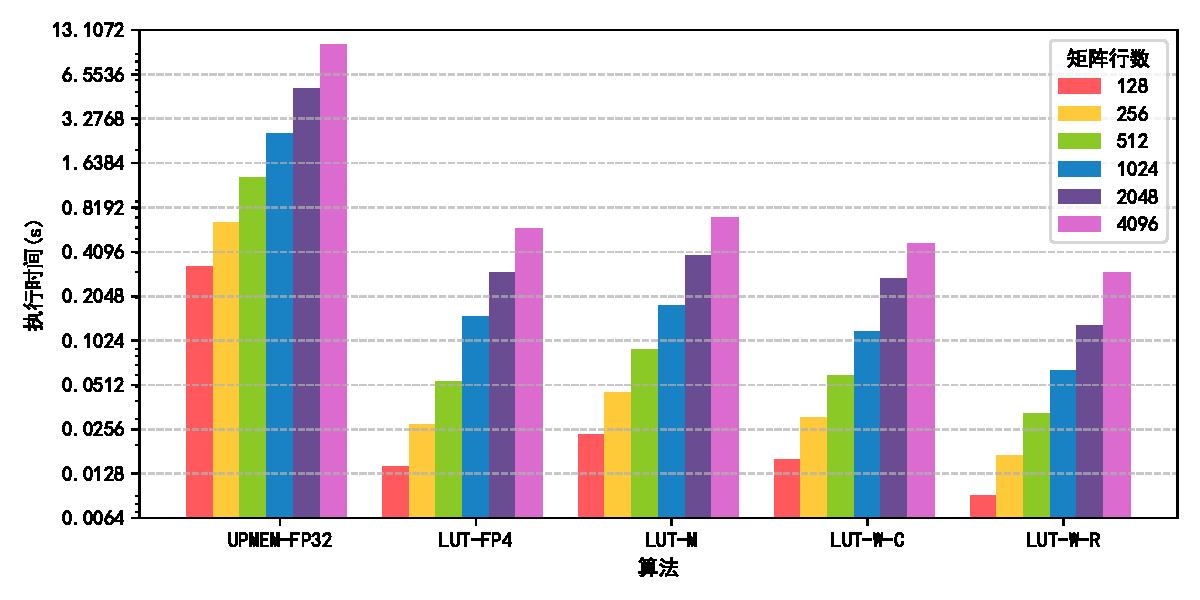
\includegraphics[width=0.45\linewidth]{figures/Exp3-2-2.pdf}
        \label{EXP3-2:2}}
	\subfigure[固定行为4096改变矩阵列]{
		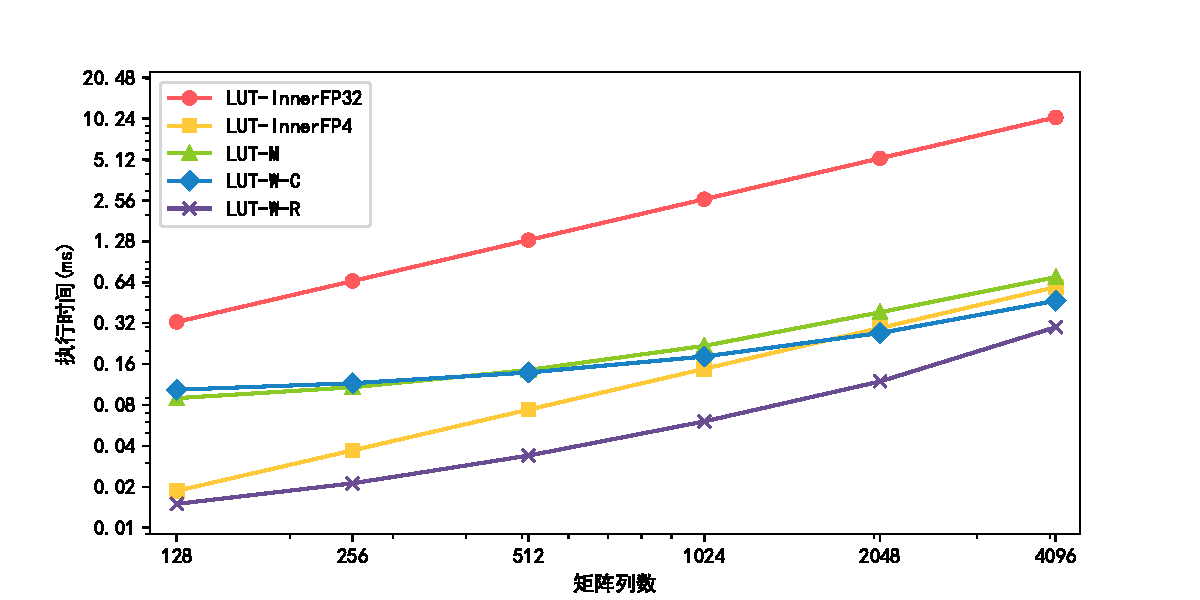
\includegraphics[width=0.45\linewidth]{figures/Exp3-2-1.pdf}
		\label{EXP3-2:1}}
	\caption{UPMEM平台不同GEMV算法矩阵尺寸扩展性测试}
	\label{EXP3-2}
\end{figure}

此外可以看到LUT-W-R在增加矩阵的列时,其执行时间并不是等比增长,而是耗时越来越多,原因在于LUT-W-R算法本身对权重矩阵的行列并不敏感,而是对其分块处理的子矩阵的大小敏感,子矩阵越大执行耗时越少。当增加矩阵的列时,会较为严重地挤占WRAM的空间导致子矩阵的变小,从而需要更多的DMA操作从MRAM中读取数据,从而造成执行耗时增加因此可以得出结论,LUT-W-R的算法更加适合行数远大于列数的“窄矩阵”,而LUT-W-C的算法更加适合列数远大于行数的“宽矩阵”。

\section{基于模拟器平台的硬件设计测试与分析}
在真实硬件平台测试后GEMV算子的各项数据后,需要对基于模拟器平台的硬件优化进行测试。我们分别做了两部分的硬件优化,分别是增加了融合查表加法指令集(FLA)和向量指令(SIMD):使用FLA指令优化第三章提出的三个基于查表的算法LUT-M、LUT-W-C和LUT-W-R;使用SIMD指令优化GEMV朴素内积LUT-FP4的算法LUT-SIMD。基于UPMEM周期精确模拟器PIMulator对上述优化进行测试,通过模拟器模拟器的周期数和主频测算算子执行耗时,进而得到算子优化后的吞吐。设置矩阵的尺寸为$4096\times 4096$,设置16个Tasklets,LUT-W-R算法配置子矩阵大小为$32\times 64$。具体的加速如图\ref{EXP2-1}所示。

\begin{figure}[!htbp]
    \centering
    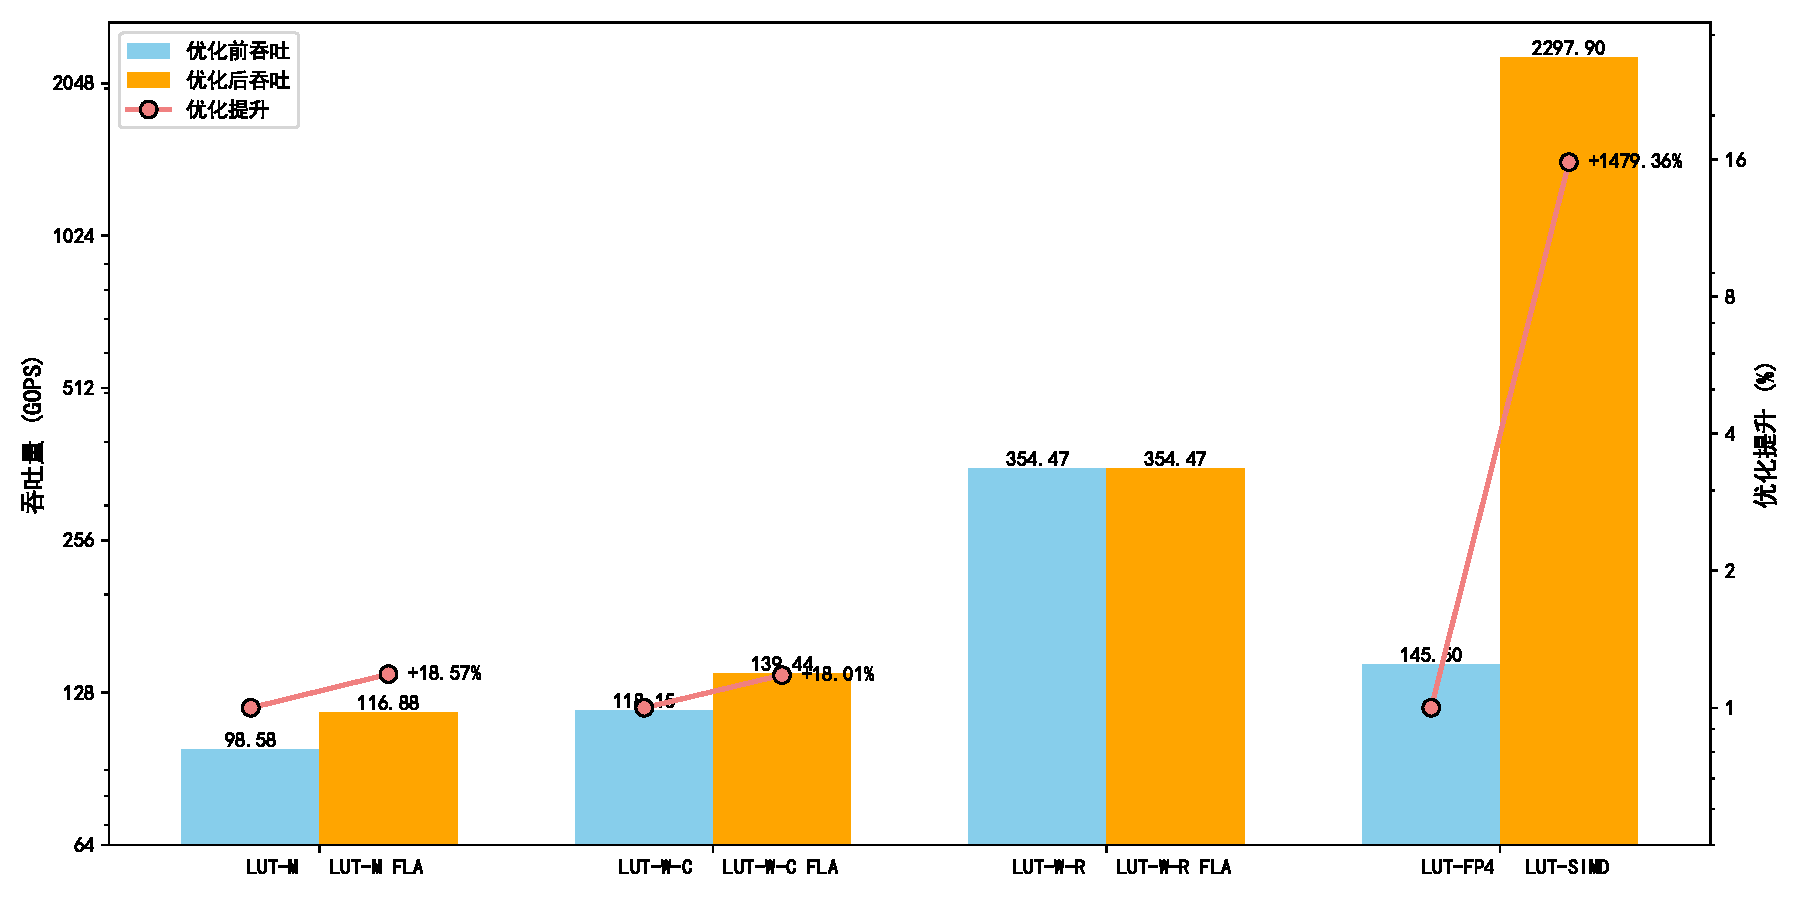
\includegraphics[width=0.9\textwidth]{figures/Exp2-1.pdf}
    \caption{硬件架构修改对于GEMV算子吞吐提升——编译优化O3}
	\label{EXP2-1}
\end{figure}

对于算法LUT-M、LUT-W-C和LUT-W-R而言,使用了FLA指令集后算子的吞吐提升分别在14.88\%、27.82\%和0\%,在这里对结果进行解释。对于LUT-M和LUT-W-C而言,提升大概在15\%~30\%左右较为优秀但是没有达到理论预期。在汇编分析的代码段\ref{LUTInstAsm}中,FMA操作的提升普遍在2~3倍,但是上述假设的情况过于理想,没有考虑寄存器的使用限制以及编译优化手段,在真实的算法汇编代码中,能够使用我们设计的查找指令的代码段仅仅在查表指令代码段一处,并且通过一定的编译优化对指令进行了重排,无法通过人手动地更改整体代码段以达到最佳优化,其结果就是使用我们设计的FLA指令往往只能优化FMA操作中的一条到两条指令:比如LUT-M仅有一处查表可以使用FLA指令增强,就是最深循环出的查表语句;而LUT-W-C算法有两处可以使用FLA指令增强,一处是查表得乘积,另一处是查表得累加索引。而我们在之前的理论最大算子吞吐的计算过程中展示过,理论上一次FMA操作往往需要消耗5条指令,因此优化大概在15\%~30\%左右符合预期。

对于算法LUT-W-R而言,我们无法通过汇编代码分析找到任何可以优化的代码段。我们分析发现LUT-W-R的算法编译优化非常好,将查表操作的额外开销部分通过指令重排优化掉了,从而导致我们无法直接从汇编代码入手优化算法,因此并无加速效果。从上面的测试可以看出,UPMEM平台的软件生态较为完善,编译优化较好,其中的部分原因可能是UPMEM本身基于RISC指令集,本身指令简单且优化成熟。然而很多其他的近存计算平台,由于底层的硬件和支持的指令集并不像UPMEM这样简单且流行,仍然存在不完善的软件链,编译优化不好的问题。因此基于上面的实验,我们做了补充实验\ref{EXP2-2},对于各个算法不开启编译优化,其余配置保持一致测试了结果。

\begin{figure}[!htbp]
    \centering
    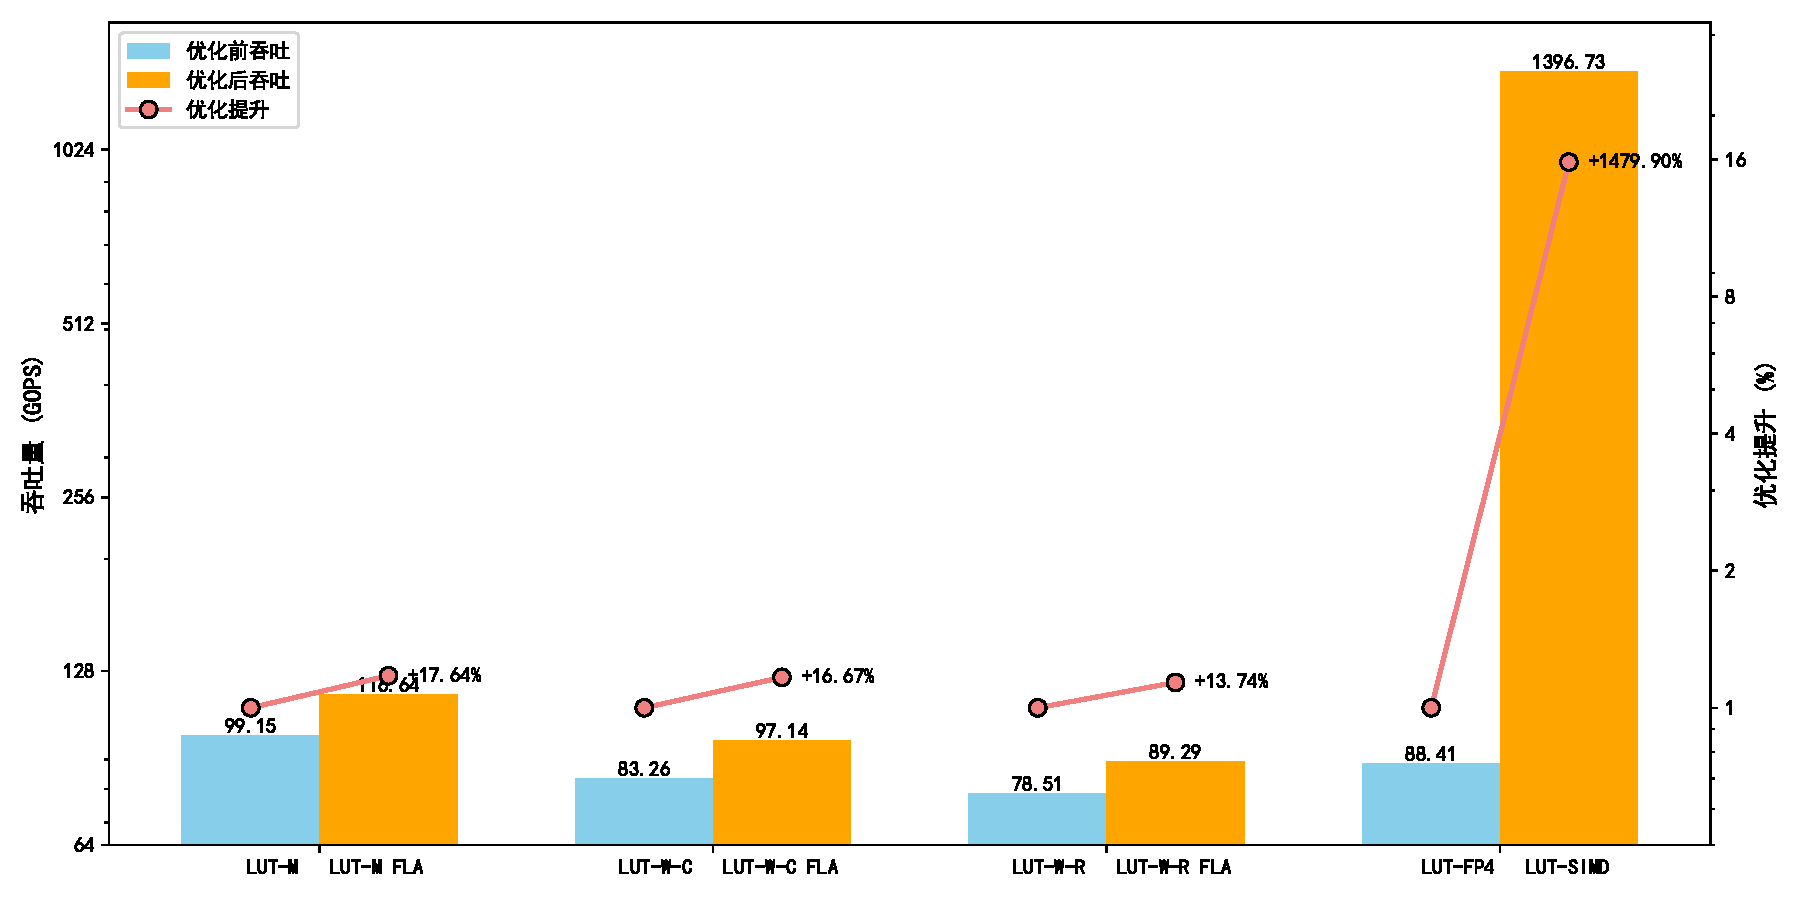
\includegraphics[width=0.9\textwidth]{figures/Exp2-2.pdf}
    \caption{硬件架构修改对于GEMV算子吞吐提升——编译优化O0}
	\label{EXP2-2}
\end{figure}

这时对于算法LUT-M,使用了FLA指令集后算子性能提升能达到17.64\%,有少许提升。算法LUT-W-C的提升为16.67\%,该算法的FLA指令增强和O3编译一样有两处,但是提升反而相比于O3编译减少了,其原因在于LUT-W-C的未经编译优化其复杂的源码结构使得其编译产生的汇编代码非常低效,吞吐量甚至低于LUT-M(LUT-W-R也是类似),并且我们在编译的汇编指令中发现了许多废指令,我们未将这些废指令或非查找表的指令优化计入,因此整体LUT-W-C的提升变低了。LUT-W-R此时就有了13.74\%的提升,提升较低的原因和其总吞吐低有关。

可以看到,对于编译优化较差的平台我们的FLA指令增强效果较好,尤其对于算法LUT-W-C,有两次随机数组访问(查表),优化效果是最好的。但是我们提出的一系列FLA指令集其实不止局限于查表的优化,可以用于多种场景,许多移位、访存和累加操作都可以通过一条FLA指令完成。此时的工作应该在编译器层面进行,直接进行汇编指令的替换不会有效果。

对于使用SIMD指令加速的效果,不论编译优化等级,比较LUT-FP4和LUT-SIMD可以发现,加速效果约为16倍(提升是1479\%差不多就是原来的16倍),这与理论提升高度符合,因为可以一次性向量完成16个元素的查表和加法,同时我们简单地修改了PIMulator模拟器的让其支持向量指令且保证CPI(Cycle Per Instruction)为1,与其他的RISC指令并无明显差异,因此原本16个元素的计算需要16次载入激活、载入矩阵、查表、累加,而使用向量指令后,就变成了1次载入子表、矩阵向量移位、重排、累加(每8次操作载入一次矩阵向量),因此性能提升非常大。

当然我们在模拟器上实现时并未考虑实际的硬件工艺和电路设计是否允许这样的支持,比如是否能够在较小的芯片内集成支持512bit向量计算的向量单元,并且能支持指令的CPI达到1。当然我们可以结合更低bit权重量化的工作减小向量的长度,比如3bit的权重量化只需要256bit的向量运算,而2bit只需要128bit。

在真实硬件平台上测试的能效比、瓶颈分析和扩展性实验,在模拟器平台上测试结论基本保持一致,在此不多赘述。

\section{本章小结}
本章对此前的软硬协同优化方案做了充分的测试及结果分析。首先介绍了测试的环境和基本配置,包括所使用的三大硬件平台的基本介绍和硬件配置,测试数据的配置以及对比基线的设置。然后在商用近存计算硬件UPMEM上做了一些的测试和分析,包括对各种基于UPMEM的优化算法的GEMV算子总吞吐测试,对比了CPU和GPU平台的算子吞吐,分析得到结论:UPMEM上GEMV算子强于CPU平台并于GPU平台持平;同时包括对三个硬件平台GEMV计算的能效比测试以及计算瓶颈分析,分析得到近存计算平台UPMEM的能效比高于CPU和GPU平台且GEMV的优化算法表现为计算瓶颈;还包括对GEMV算子的扩展性测试,测试得到此前提出的GEMV算法对于Tasklet有良好的扩展性(不超过11个线程),而对于矩阵的尺寸大多也同样具有良好的扩展性,其中LUT-M和LUT-W-C算法更适合在行数远小于列数的矩阵,而LUT-W-R则更适合行数远大于列数的矩阵。最后在PIMulator模拟器上测试硬件的修改对于GEMV算子性能的提升,其中增加FLA指令集对于LUT-M和LUT-W-C的提升在15\%~30\%左右,增加向量处理单元对于LUT-FP4算法的提升在16倍。